\subsection{Overview}

\subsection{Component View}
\begin{figure}[H]
    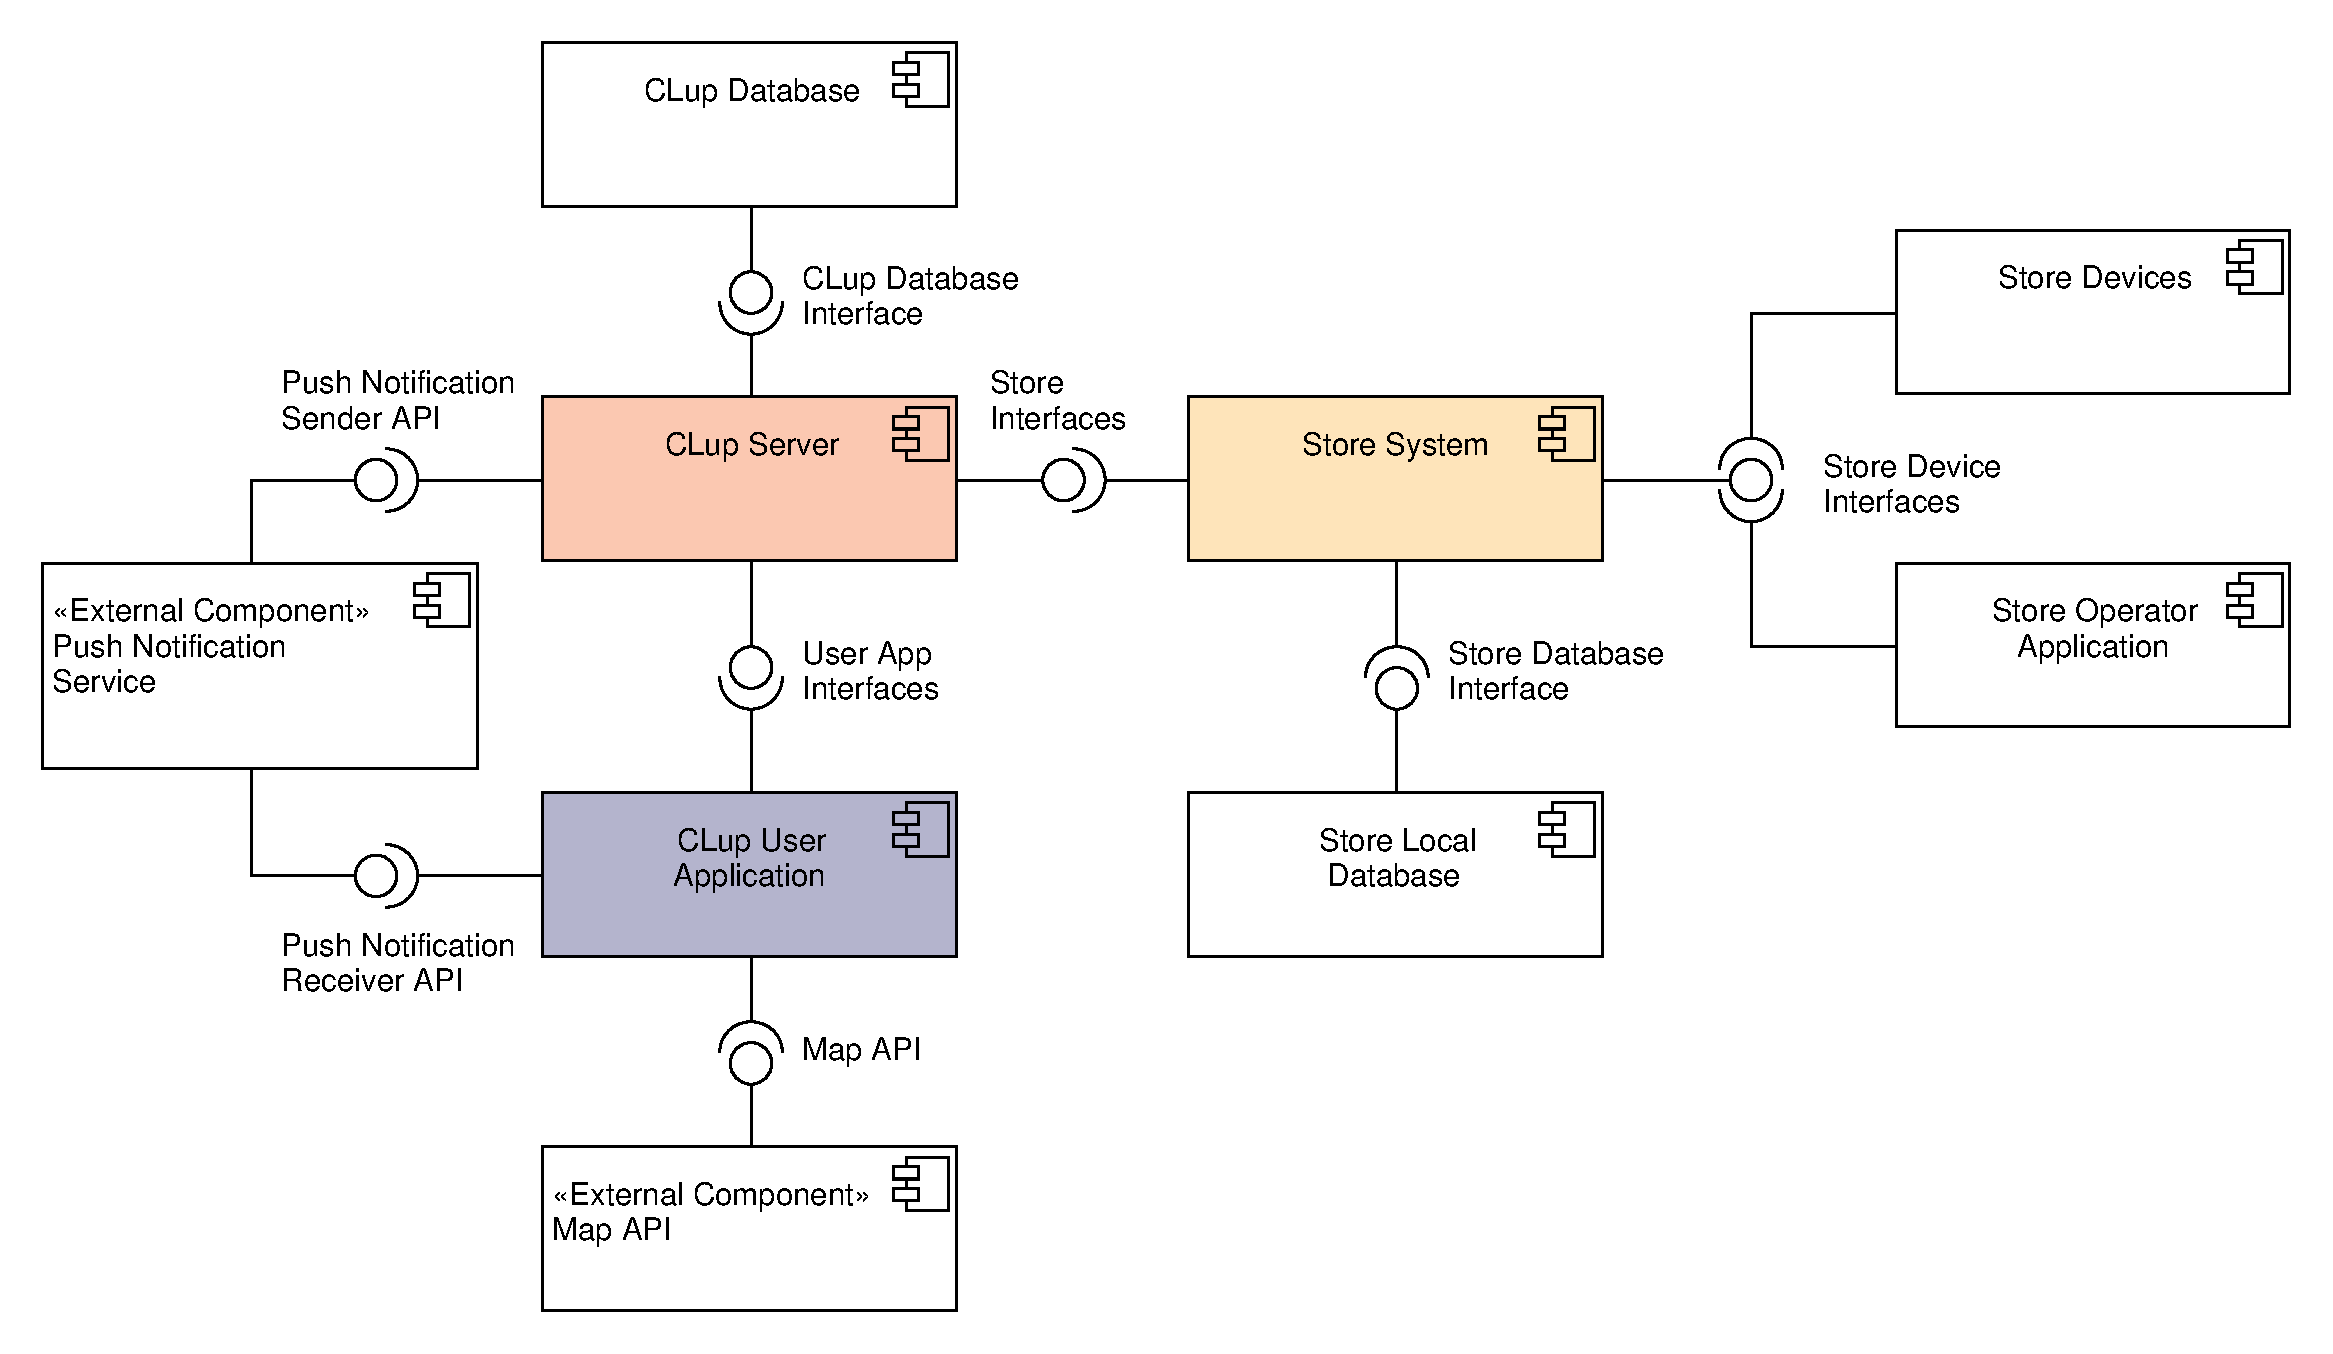
\includegraphics[width=\textwidth]{Images/UML_general_component.pdf}
    \caption{\label{fig:UML_comp_general}General component diagram}
\end{figure}
In the figure~\ref{fig:UML_comp_general} is shown a general simplified component view of the S2B.
The three main components of the system are the CLup User Application, the CLup Server and the Store System with their databases. The system includes also external components like a Map Service and other physical components (i.e.~store devices).

Customer use the \textbf{CLup User application} to check supermarket near them and eventually book a visit
or retrieve a ticket. The User application interfaces with the \textbf{CLup server} 

The CLup server is the
central point of the system, mediating between the customer and the store. It manages customer authentication, 
tickets issued remotely from the CLup application, and hands out to the public information about the store to the customers 
(i.e.~opening hours, waiting times\ldots).

The Store system provides an interface for all the physical devices in the store, collecting and processing data from them 
and then routing data to the CLup server or keeping it in the local database. The system communicates with a local database keeping in it temporary data about tickets, the statistics collected and the 
authentication details of the store operators.

\subsubsection{CLup Server component view}
\begin{figure}[H]
    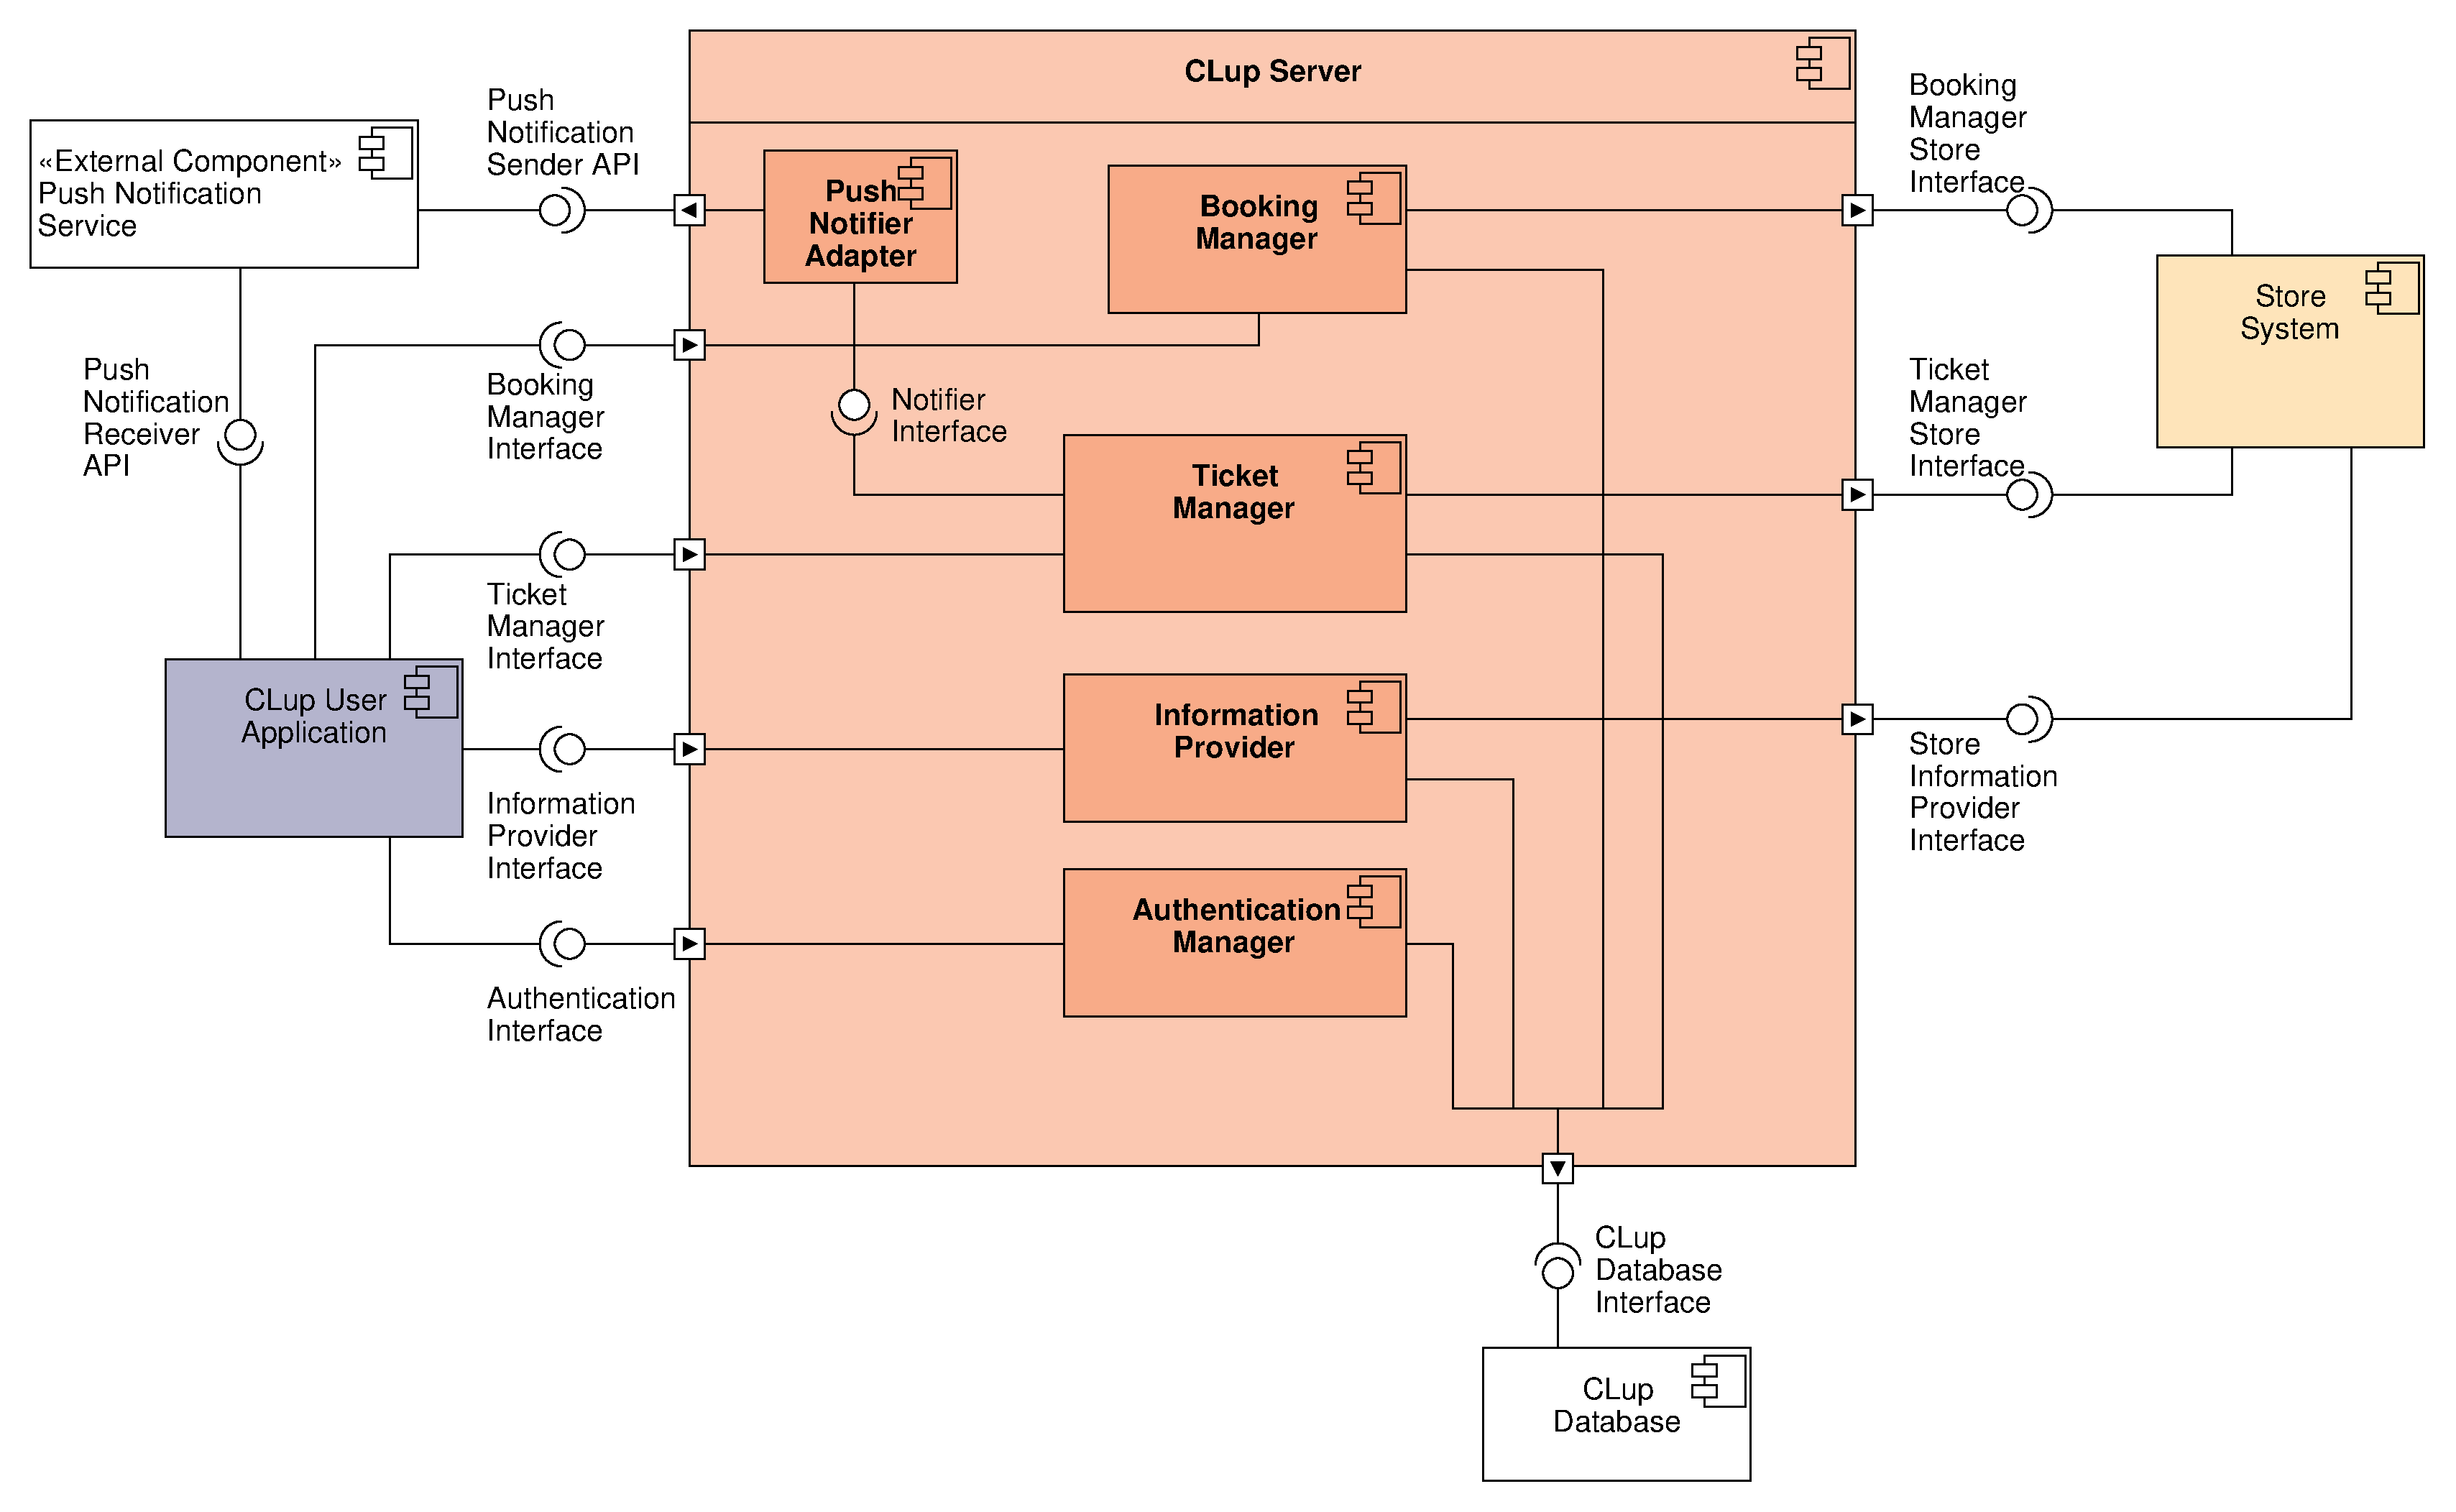
\includegraphics[width=\textwidth]{Images/UML_server_component.pdf}
    \caption{\label{fig:UML_comp_Clup_server}Component diagram for CLup server}
\end{figure}

The CLup server provides interfaces either to the CLup User applications either to each store system. This component store the persistent data in the CLup Database component communicating to it using a common Database interface.

The CLup system has these internal components:
\begin{itemize}
    \item Authentication Manager: Handles the customer registration and authentication. To do this task this component need to communicate tightly with the CLup database that stores the user data and their passwords
    \item Information Provider: Hands out information to the customer requesting them. These information could be of various nature like opening hours or the store crowdedness in various time of the day. This component retrieves these data are retrieved from the CLup database or from the store system that uses and interface to push them periodically.
    \item Ticket Manager: Issues a virtual tickets when the customer requires it. This component interfaces directly with the store adding the created ticket to the queue. The component has the responsibility to notify the customer when it's time to approach the store entrance using the notifier interface, provided from the notifier component.
    \item Booking Manager: Handles the visit booking. Queries the database about free slots in the day when the customer wants to book. The components also manages and finalizes the request attaching eventually the shop list to the booking when the customer adds it. This components sends updates to the store system about the bookings.
    \item Notifier: Handles all the aspects about sending push notifications to the users, taking in account the fact that different operating systems where the CLup customer application is installed provides a different system interface to receive these notifications. 
\end{itemize}

\subsubsection{CLup customer application component view}
\begin{figure}[H]
    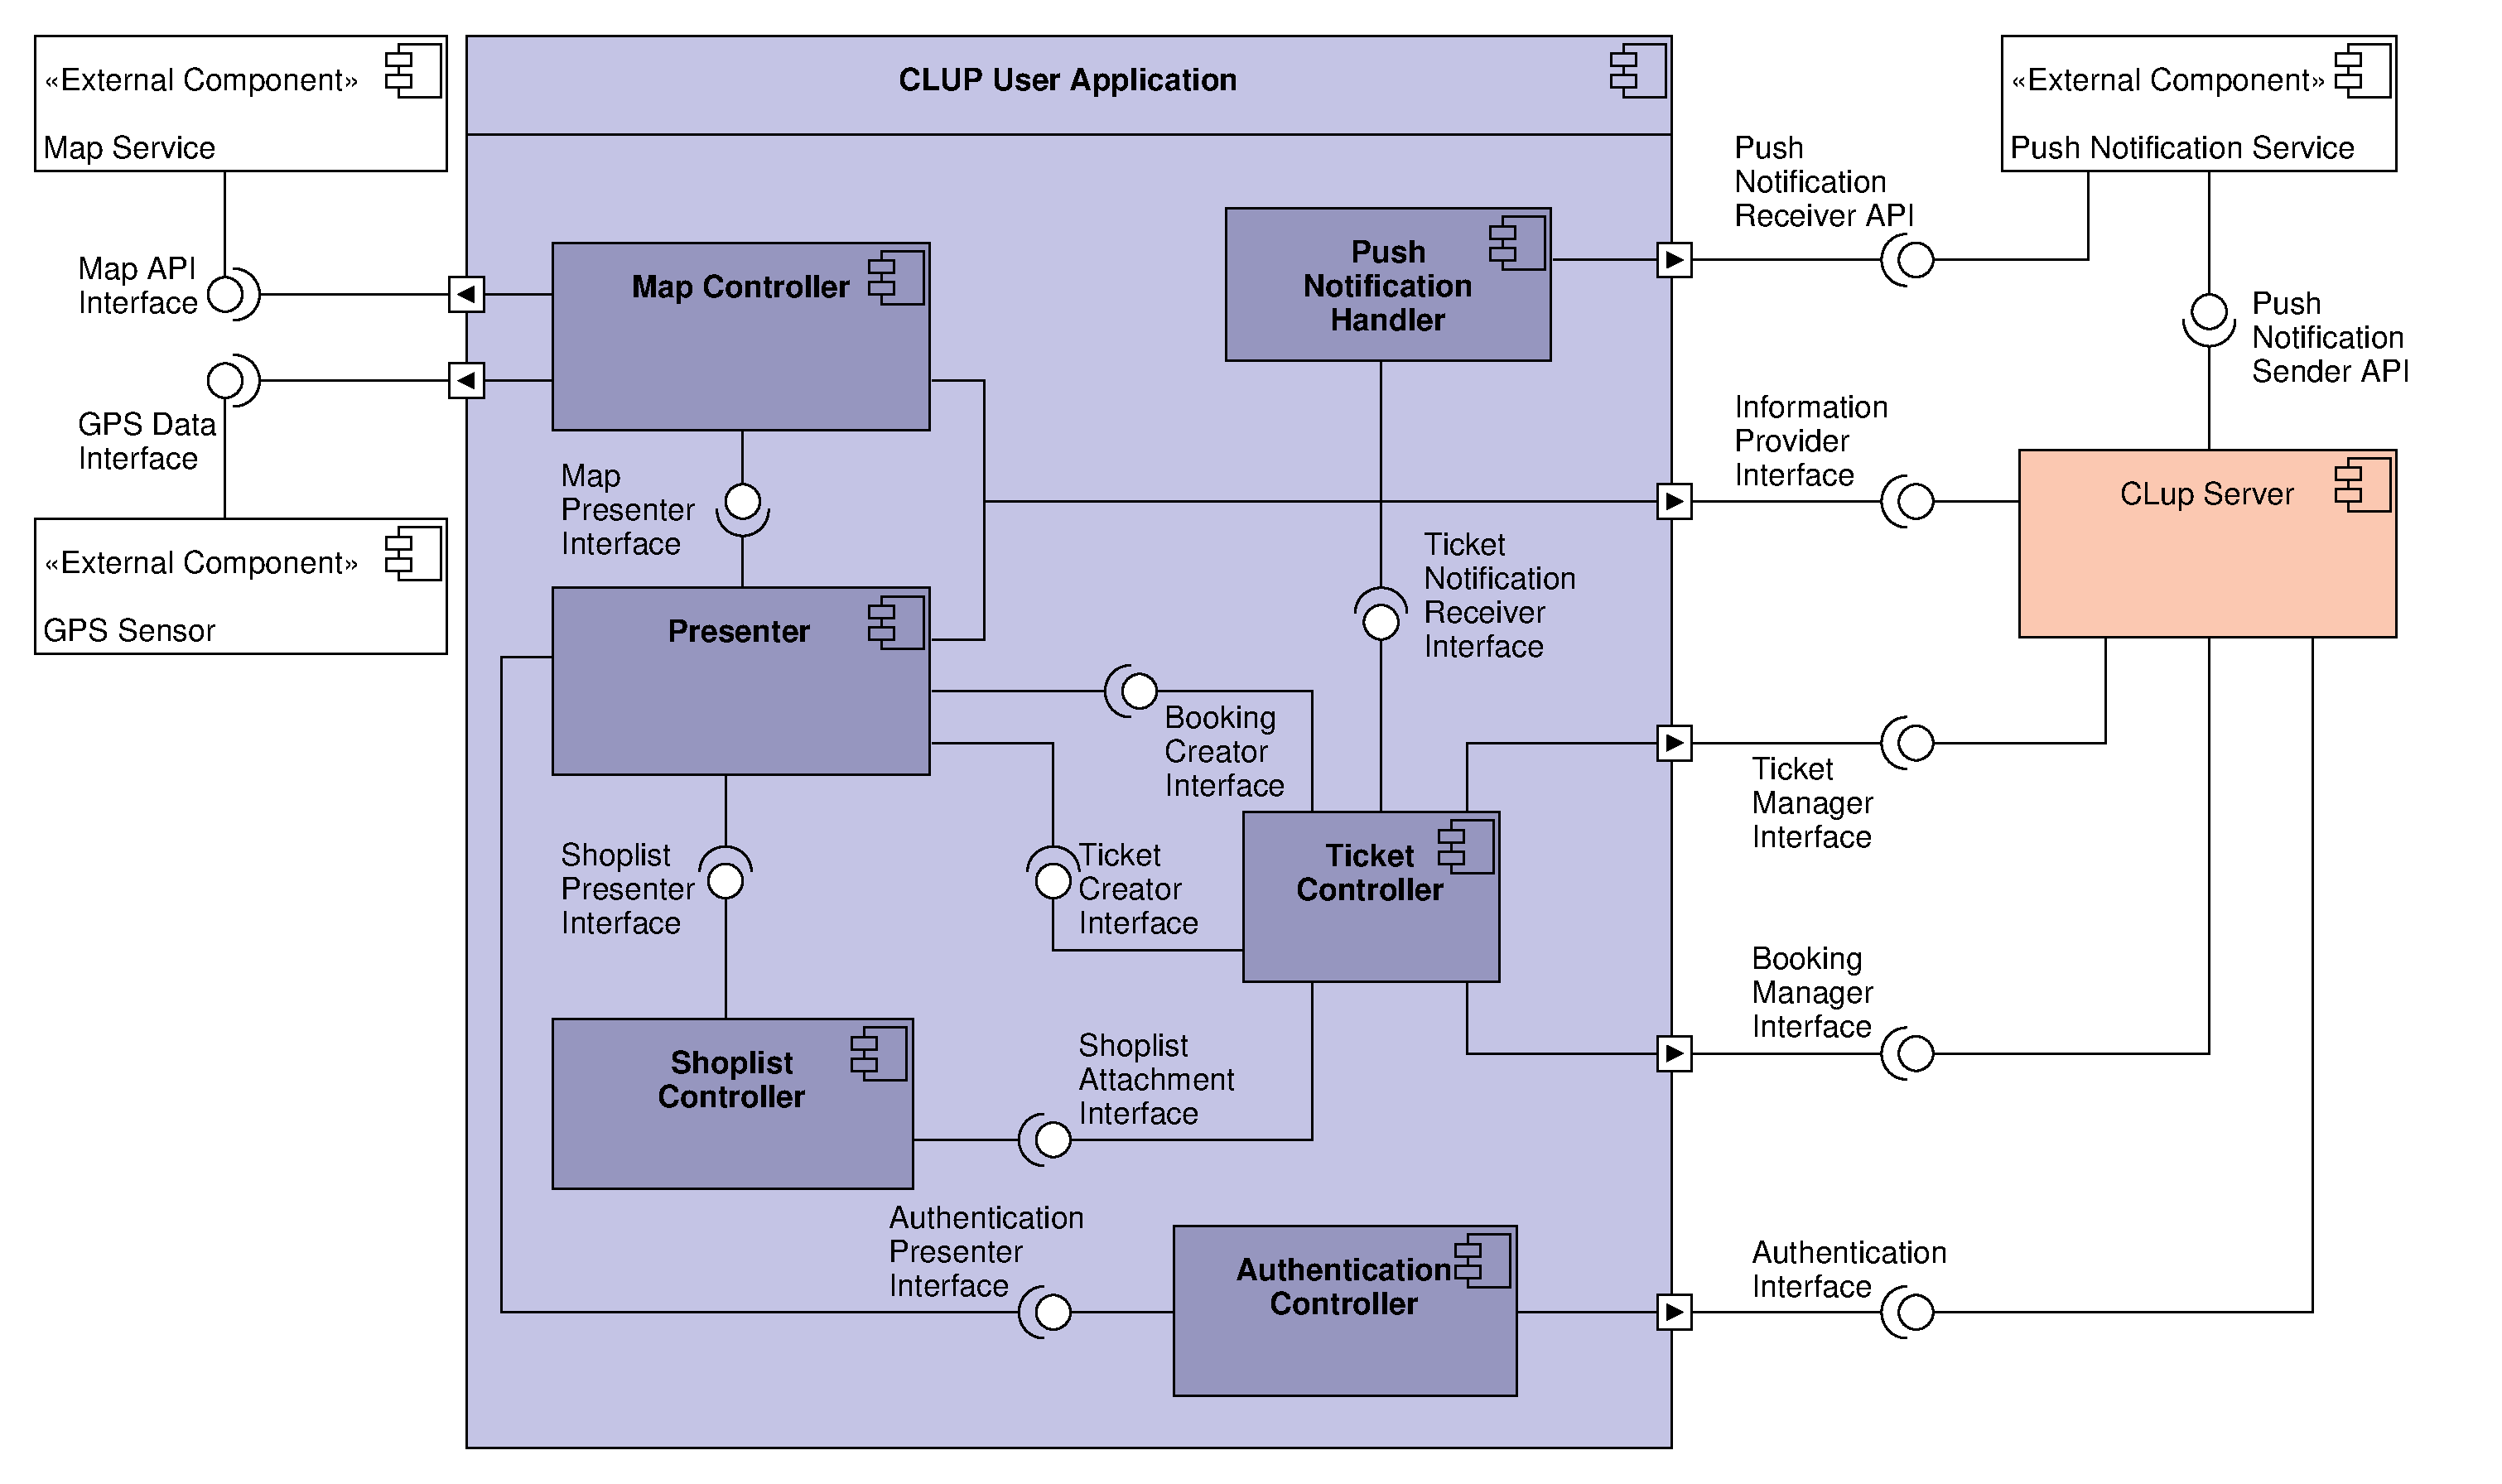
\includegraphics[width=\textwidth]{Images/UML_user_app_component.pdf}
    \caption{\label{fig:UML_comp_CLup_user_app}Component diagram for CLup User Application}
\end{figure}

The CLup user application provides the functionalities of the CLup to the store's customers. The applications needs to interface to the GPS Sensors and to an external map service to provide a map containing all the stores. The application needs also some controllers that will communicate with the CLup server to retrieve store information, authenticate and book a visit or issue a ticket.

The user application contains these sub components:
\begin{itemize}
    \item Authentication: allows the user to create a CLup account and to log-in in an existing account.
    \item Map Controller: Handles the first screen that the user will se after logging in. Naturally it needs to use the Map API provided from the Map Service and needs to access data about the position of the user. It also needs to query the CLup server in order to get all the supermarkets position and display them as waypoints in the map, for this task the component will use the Information provider Interface offered from the CLup server component. Finally when a supermarket is selected the Shop Information presenter component interface calls will be used.
    \item Store information presenter: shows in an user friendly way essential information about a store (i.e. Store address, Opening hours, crowdedness, estimated waiting times) using the information provider interface. This component allows the creations of bookings directly from the store page calling the Ticket Controller's Booking Creator Interface methods.
    \item Shop-list controller: manages the creation of a shop list that will be attaches to a visit booking in order to estimate the occupancy of the various department of the store
    \item OS notifications handler: handles and displays to the user the push notification received from the CLup Server about the bookings or the tickets created from the user. Each OS where the application handles these notifications in a slightly different way, this component must take in consideration this fact.
\end{itemize}

\subsubsection{Store System component view}
\begin{figure}[H]
    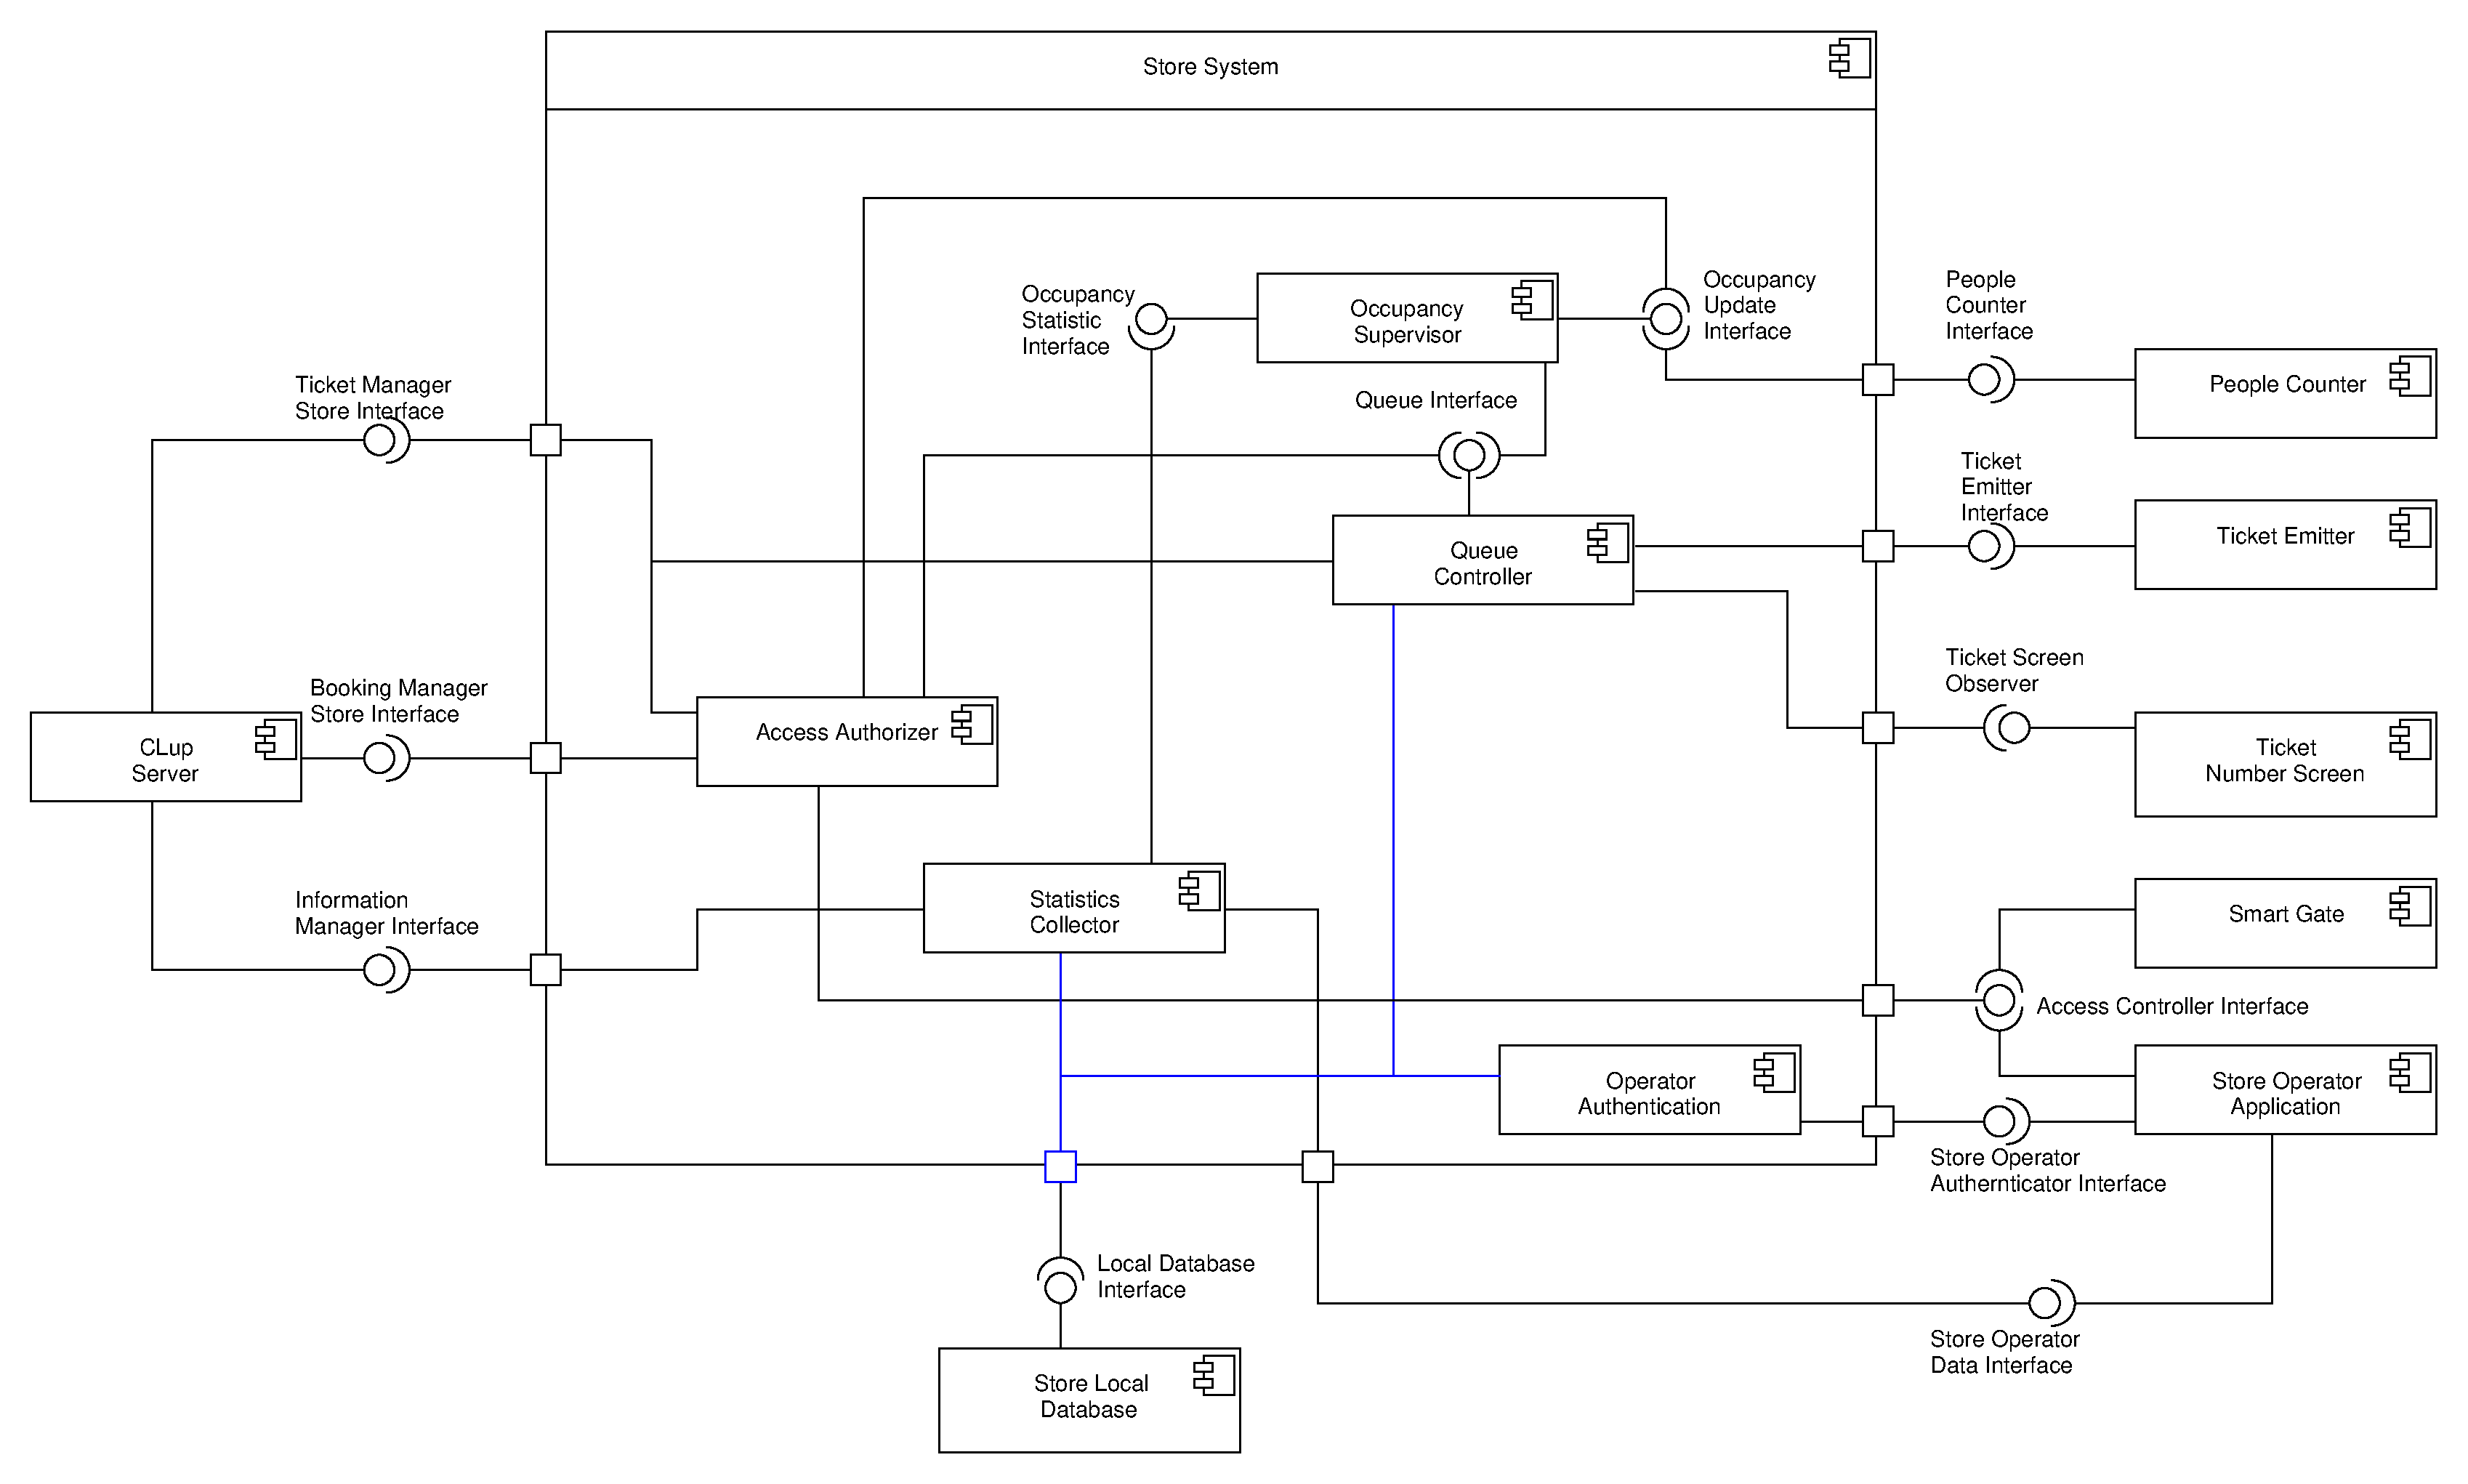
\includegraphics[width=\textwidth]{Images/UML_store_system_component.pdf}
    \caption{\label{fig:UML_comp_CLup_store_system}Component diagram for Store system}
\end{figure}

The Store system receives data from the store physical devices that collect data and combined with the data retrieved from the CLup servers actuates and implement the CLup system store part. This component uses the interfaces provided from the CLup server and provides interfaces used from to the physical devices located in the store. This component interfaces with a local database containing store statistics, store operator authentication data and local data that need persistency.

\begin{itemize}
    \item Operator Authentication: allows the store operator to authenticate using their store credential. This component communicates with the Store Operator Applications used to check the tickets and register the customer admissions to the store. The component fetches the authentication data in the store local database, using the interface provided from the database.
    \item Occupancy Supervisor: checks that the occupancy limits are not violated using all the data that receives about people entering and leaving the store. Those data could be provided directly from devices People Counters, or from the Access Authorizer that increment the number of people inside the store when an access is authorized. The occupancy supervisor checking information about the bookings notifies the queue controller when there is space to admit customers with a numbered ticket (without a booked visit).
    \item Queue Controller: handles the queueing of the customers retrieving data regarding the virtual numbered ticket from the CLup server and data regarding the paper numbered ticket from the ticket emitter, using the proper interfaces. The queue controller is notified from the occupancy supervisor when some customers in line could be called to the entrance and then updates the ticket number screen placed at the store entrance with the new number called using his interface.
    \item Access authorizer: receives the code read from the Access controller (that could be either a Smart Gate or a store operator) checks if that code is valid and allowed to enter, then notifies back the access controller. Even if the ticket is valid before admitting a customer this component needs to check that the occupancy limits of the store will not be violated if another customer is admitted consulting the Occupancy Supervisor. This component will check the CLup server if the ticket refers to a pre booked ticket, in the other cases the access controller will check if the ticket is on top of the queue using the Queue controller interface. 
    \item Statistics Collector: collects and elaborates periodically statistics from the Occupancy Supervisor, Queue Controller and stores it in the store local database. Brief elaborated data that could is shown to the customer (i.e.~indications of the crowdedness of the store, estimated waiting times\ldots) are sent periodically to the CLup Server using the Store Information Provider Interface.  
\end{itemize}
\subsection{Deployment View}

\subsection{Runtime View}

\subsection{Component Interfaces}

\subsection{Style Architecture}

% TODO: add section about relevant interfaces and algorithms is pseudocode